In \cite{peres1990incompatible,mermin1990simple}, Mermin and Peres discovered an algebraic coincidence related to the $3\times3$ ``Magic Square'' of operators on $\C^2\otimes \C^2$ in Figure \ref{fig:magic-square-operators-introduction}.

If we pick any row and take the product of the three operators in that row (note that they commute, so the order does not matter), we get the identity operator. Similarly, we can try this with the columns. Two of the columns give identity while the other  gives $-1$ times identity. Thus, the product of these nine operators depends on whether they are multiplied row by row or column by column. This can be exploited to define a two-player, one-referee game called the Mermin--Peres Magic Square game \cite{aravind2004quantum} (see Definition \ref{definition:linear-constraint-game} and Figure \ref{fig:magic-square-equations} for a formal definition). Informally, the Mermin--Peres Magic Square game mod $2$ is as follows. The players claim to have a $3\times 3$ square of numbers in which each row and each of the first two columns sums to $0\pmod 2$, while the third column sums to $1\pmod 2$. (The players are usually called ``provers'', since they try to prove that they have such a square.) The referee asks the first player to present a row of the supposed square and the second to present a column. They reply respectively with the $3$ entries of that row and column in $\{0,1\}$. They win if their responses sum to $0$ or $1$ as appropriate, and they give the same number for the entry where the row and column overlap. This game can be won with probability $1$ by provers that share two pairs of maximally entangled qubits of dimension $2$, but provers with no entanglement can win with probability at most $\frac89$. Games which are won in the classical case with probability $< 1$ but are won in the quantum case with probability $1$ are known as \emph{pseudotelepathy games}.


\begin{figure}[!b]
	\caption{On the left are the operators of the Magic Square. $X$ and $Z$ are the generalized Pauli operators, i.e. they are unitaries for which $X^2 = Z^2 = I$ and each permutes the eigenbasis of the other. Across any solid line, the three operators commute and their product is identity. Across the dashed line, the operators commute and their product is $-1$ times identity.}
	\label{fig:magic-square-operators-introduction}
	\begin{tabular}
		{m{0.5\textwidth}m{0.5\textwidth}}
		  \resizebox{0.5\textwidth}{!}{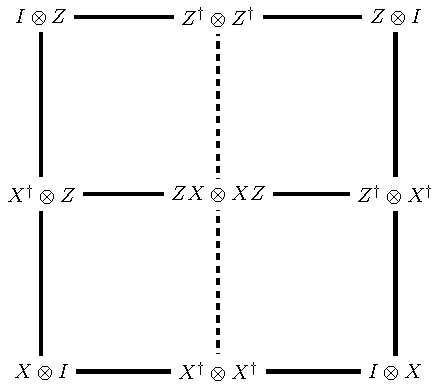
\includegraphics{MagicSquare-figure0.pdf}}
		 &\resizebox{0.5\textwidth}{!}{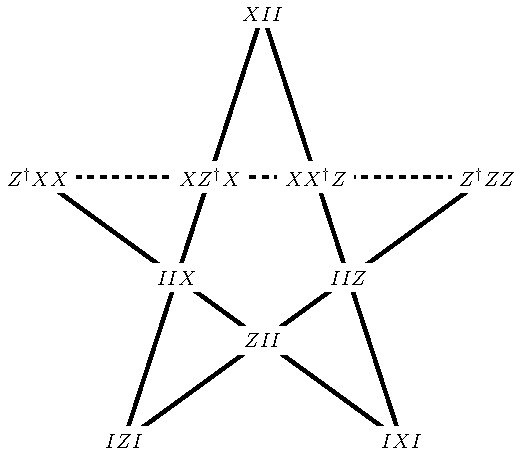
\includegraphics{MagicSquare-figure1.pdf}}
	\end{tabular}
	\caption{On the right are the operators of the Magic Pentagram. These are operators on $(\C^2)^{\otimes 3}$; the tensor product symbols are omitted. Across any line, the four operators commute. Across any solid line, the alternating product $AB^\dagger CD^\dagger$ of the four operators is identity. Across the dashed line, the alternating product (computed from left to right) is $-1$ times identity.}
	\label{fig:magic-pentagram-operators-introduction}
\end{figure}

How special is this ``algebraic coincidence'' and the corresponding game? We can refine this question into a few sub-questions.
\begin{question}\label{question:is-magic-square-setup-unique?}
	% Are there other sets of algebraic relations that give rise to interesting games?
	Are there other configurations of operators with similarly interesting algebraic relations? Do they also give rise to pseudotelepathy games?
\end{question}

Arkhipov \cite{arkhipov2012extending} gives a partial answer to this question by introducing the framework of \emph{magic games}. Starting from any finite graph, one can construct a magic game similar to the Magic Square game. Arkhipov finds that there are exactly two interesting such magic games: the Magic Square (derived from $K_{3,3}$, the complete bipartite graph with parts of size $3$) and the Magic Pentagram (derived from $K_5$, the complete graph on $5$ vertices). 
Subsequently, Cleve and Mittal \cite{cleve2014characterization} introduced \emph{linear constraint system games} (hereafter referred to as \emph{LCS games}), which can be thought of as a generalization of Arkhipov's magic games from graphs to hypergraphs. Moreover, they proved that any linear constraint game exhibiting pseudotelepathy requires a maximally entangled state to do so. Their result also suggested that there may be other interesting linear constraint games to find. Indeed, Ji showed \cite{ji2013binary} that there are families of linear constraint games requiring arbitrarily large amounts of entanglement to win. 


\begin{question}\label{question:is-magic-square-solution-unique?}
	The easiest proof of correctness for a Magic Square game strategy uses the fact the observables measured by the players satisfy the appropriate algebraic relations. Is this a necessary feature of any winning strategy?
\end{question}

In order to answer questions like this, Cleve, Liu, and Slofstra \cite{cleve2016perfect} associate to each LCS game an algebraic invariant called the \emph{solution group} (see Section \ref{sec:linear-constraint-games} for a precise definition), and they relate the winnability of the game to the representation theory of the group. In particular, they show that any quantum strategy winning the game with probability $1$ corresponds to a representation of the solution group---in other words, that the observables in a winning strategy must satisfy the algebraic relations captured by the group. This reduces the problem of finding LCS games with interesting properties to the problem of finding finitely-presented groups with analogous representation-theoretic properties, while maintaining combinatorial control over their presentations. Slofstra used this idea together with techniques from combinatorial group theory to resolve the weak Tsirelson problem \cite{slofstra2016tsirelson}. By including some techniques from the stability theory of group representations, he improved this result to show that the set of quantum correlations is not closed \cite{slofstra2017set}. In words, he constructed an LCS game which can be won with probability arbitrarily close to $1$ with finite-dimensional quantum strategies, but cannot be won with probability $1$ by any finite (or infinite) dimensional quantum strategy (in the tensor product model).


\begin{question}\label{question:is-magic-square-game-rigid}
	We introduced the magic square operators and then noticed that they satisfy certain algebraic relations. Do these algebraic relations characterize this set of operators? Could we have picked a square of nine different operators, possibly of much larger dimension, satisfying the same relations?
\end{question}

This question was resolved by Wu et.\ al \cite{wu2016device}. They showed that any operators satisfying the same algebraic relations as those in the Magic Square game are equivalent to those in Figure \ref{fig:magic-square-operators-introduction}, up to local isometry and tensoring with identity. This is sometimes referred to as \emph{rigidity} of the Magic Square game. Moreover, they showed that the Magic Square game is \emph{robustly rigid}, or \emph{robustly self-testing}. Informally, we say that a game is \emph{rigid with $O(\d(\e))$-robustness and perfect completeness} if whenever Alice and Bob win the game with probability at least $1-\e$, then there is a local isometry taking their state and measurement operators $O(\d(\e))$-close to an ideal strategy, possibly tensored with identity.

%\footnote{We'll measure this closeness in a state-dependent distance given in Equation \ref{eq:state-dependent-distance-definition}.} up to local isometry and tensoring with identity, to the ideal strategy. 

\paragraph{Our contributions}
Our main result is a robust self-testing theorem which applies to any linear constraint game with sufficiently nice solution group; this is stated as Theorem \ref{thm:robust-self-testing}. Our proof employs the machinery of \cite{cleve2016perfect} and \cite{slofstra2016tsirelson}. We apply the general self-testing result to conclude robust rigidity for the Magic Square game, the Magic Pentagram game, and for a certain repeated product of these two games. We informally state these results now. We emphasize that these results are not new, but it is new that we can achieve all three as simple corollaries of the main self-testing machinery. The general result holds for LCS games mod $d$, but the only nontrivial application we have is for LCS games mod $2$.

\begin{thm}[Informal, c.f. Definition \ref{defn: robust-self-testing} and Theorem \ref{thm:robust-self-testing-square}]\label{thm:informal-magic-square}
	The Magic Square game is rigid with $O(\e)$-robustness and perfect completeness. The ideal state is two copies of the maximally entangled state of local dimension $2$, and the ideal measurements are onto the eigenbases of the operators in Figure \ref{fig:magic-square-operators-introduction}.
\end{thm}
\noindent
This recovers the same asymptotics as in \cite{wu2016device}. Note that they state their robustness as $O(\sqrt\e)$; this is because they use the Euclidean distance $\norm{\ket\psi - \ket{\text{ideal}}}$, while we use the trace-norm distance of density operators $\norm{\rho - \rho_{\text{ideal}}}_1$. 

\begin{thm}[Informal, c.f. Theorem \ref{thm:robust-self-testing-pentagram}]\label{thm:informal-magic-pentagram}
	The Magic Pentagram game (see Figure \ref{fig:magic-pentagram-equations} for a definition) is rigid with $O(\e)$-robustness and perfect completeness. The ideal state is three copies of the maximally entangled state of local dimension $2$, and the ideal measurements are onto the eigenbases of the operators in Figure \ref{fig:magic-pentagram-operators-introduction}.
\end{thm}
\noindent
This recovers the same asymptotics as \cite{kalev2017rigidity}, up to translation between distance measures.

% To the best of the authors' knowledge, the only previous results for self-testing maximally (or partially) entangled qudits of any dimension $d\neq 2^n$ are those of \cite{CGS16} and \cite{CS17}. Note, however, that these are phrased in terms of correlations, while we provide the first examples where this is achieved via a nonlocal game.\footnote{The difference between a nonlocal game and a correlation lies in the amount of work required by the verifier. For the former, the verifier need only check a binary win condition which the provers aim to satisfy as often as possible. In the latter, the verifier must compare the output distribution of the provers to some ideal distribution. This may in principle require exponentially many samples to achieve the desired precision, since some answers may be required to have small positive probability of appearing.} 
Applying our general self-testing theorem to the LCS game product
\footnote{This is defined precisely in Definition \ref{def:lcs-game-product}. This is similar to but not the same as playing multiple copies of the game in parallel.} 
of many copies of the Magic Square game yields a self-test for $n$ maximally entangled pairs of qubits and associated $n$-qubit Pauli measurements. 

\begin{thm}[Informal, c.f. Theorem \ref{thm:self-testing-pauli-LCS}]\label{thm:informal-n-qudit-pauli-self-testing}
	For any $n\geq 2$, there is a linear constraint system game with $O(n^2)$ variables, $O(n^2)$ equations, and $\Z_2$-valued answers which is rigid with $O(n^{10}\e)$-robustness and perfect completeness.
	The ideal state is $n$ copies of the maximally entangled state of local dimension $2$. The ideal measurements are onto the eigenbases of certain Pauli operators of weight at most $5$. 
\end{thm}
The polynomial scaling in $n$ is similar to previous works that self-test $n$ pairs of maximally entangled qubits via copies of the magic square game \cite{coladan17, CN16}, but we obtain our bound by a simple application of our general self-testing theorem. 
% On the other hand, the polynomial scaling in $d$ is also comparable to previous robustness bounds for testing entangled qudits for any $d$ (in the $n=1$ case) \cite{CS17}. The authors believe that robustness scaling polynomially in $d$ and $n$ is necessary for any LCS game testing $n$ pairs of maximally entangled qudits. It may be possible to improve on the exponents.

\tocless\subsection{Proof Overview}
We step away from games and back towards algebra to discuss Question \ref{question:is-magic-square-game-rigid}. Suppose we wanted a $3\times 3$ square of operators, call them $e_1$ through $e_9$, with the same relations as those in the Magic Square. Concretely, those relations are as follows:\\
\begin{tabular}
	{m{0.2\textwidth}m{0.6\textwidth}}

	  \resizebox{0.2\textwidth}{!}{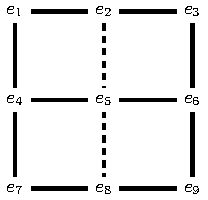
\includegraphics{MagicSquare-figure2.pdf}}
	& \begin{itemize}
		\item The linear constraints of each row and column: $e_2e_5e_8 = -I$,
		$e_1e_2e_3 = e_4e_5e_6 = e_7e_8e_9 = e_1e_4e_7 = e_3e_6e_9 = I$. 
		\item Commutation between operators in the same row or column: $e_1e_2 = e_2e_1$, $e_1e_3 = e_3e_1$, $e_2e_3=e_3e_2$, \ldots,
		$e_3e_6 = e_6e_3$, $e_3e_9=e_9e_3$, $e_6e_9=e_9e_6$.
		\item Associated unitaries have $2$ eigenspaces: $e_i^2= I$ for all $i$.
	\end{itemize}
\end{tabular}

These are just multiplicative equations. We can define an abstract \emph{group} whose generators are the $e_i$ and whose relations are those above. This is, in a sense, the most general object satisfying the Magic Square relations. More precisely, any square of operators satisfying these relations is a \emph{representation} of this group. 
It's not hard to compute that this group is isomorphic to the group of two-qubit Pauli matrices, a friendly object. (This is proven as Proposition \ref{prop:solution-group-square}.) 
This group is the \emph{solution group} of the magic square game. We study the representation theory of the solution group of the magic square game, and we apply \cite{cleve2016perfect} to deduce the exact version of our self-testing Theorem \ref{thm:informal-magic-square} (i.e. the $\e=0$ case). One might view our proof via solution groups as an ``algebrization'' of the proof in \cite{wu2016device}.

%For odd $d$, this solution group turns out to be abelian, which implies that classical players can do just as well as quantum players. 
% This algebrization admits us to easily replace $\Z_2$ with $\Z_d$ for any $d$.

In order to get the robustness bounds, we must work significantly harder. Tracing through the proof of the main result of \cite{cleve2016perfect}, a finite number of equalities between various operators are applied. Knowing how many equalities are needed, one can get quantitative robustness bounds by replacing these with approximate equalities and then applying finitely many triangle inequalities. In order to carry out this counting argument, we introduce a measure of complexity for linear constraint games and then upper bound the robustness parameter as a function of this complexity.

This complexity measure depends on the use of van Kampen diagrams, a graphical proof system for equations in finitely-presented groups. Van Kampen diagrams are introduced in \S \ref{subsection:van-kampen-diagrams}. Several of our main proofs reduce to reasoning visually about the existence of such diagrams.
Manipulating the chains of approximate equalities requires us to develop familiarity with a notion of state-dependent distance; this is done in \S \ref{subsection:state-dependent-distance}.


% \tocless\subsection{Open Problems}

\tocless\subsection{Organization}

In Section \ref{sec:preliminaries}, we establish basic tools that we'll use without comment in the main body of the paper. In Section \ref{sec:linear-constraint-games}, we give the definition and basic properties of linear constraint games over $\Z_d$. Those familiar with linear constraint games over $\Z_2$ will not find surprises here. In Section \ref{sec:self-testing}, we establish our measure of LCS game complexity and prove our general robust self-testing result, Theorem \ref{thm:robust-self-testing}. We warm up first by proving the $\e=0$ case of the theorem in \S\ref{subsection:exact-self-testing}. We then introduce two new ingredients to obtain a robust version. In \S\ref{subsection:stability-lemma}, we give a proof by Vidick \cite{vidick2017approx} of a so-called \emph{stability theorem for representations of finite groups} (Lemma \ref{lemma:vidick-gowers-hatami}). Such a result first appeared in \cite{gowers2015inverse}. In \S\ref{subsection:quant-van-kampen}, we show how to extract quantitative bounds on lengths of proofs from van Kampen diagrams, and in \S\ref{subsection:robust-self-testing}, we complete the proof of the general case. In Section \ref{sec:specific-games}, we specialize our robust self-testing theorem to the case of the Magic Square and Magic Pentagram games, establishing Theorems \ref{thm:robust-self-testing-square} and \ref{thm:robust-self-testing-pentagram}. We go on to exhibit a way to compose LCS games in parallel while controlling the growth of the complexity, proving Theorem \ref{thm:self-testing-pauli-LCS}.
